\documentclass[12pt]{article}

% report, book

%  Русский язык

\usepackage[T2A]{fontenc}
\usepackage[utf8]{inputenc}
\usepackage[english,russian]{babel}

\usepackage{amsmath,amsfonts,amssymb,amsthm,mathtools} 
\usepackage{float}

\usepackage{graphicx}
\usepackage{listings}
\usepackage{hyperref}
\usepackage[table,xcdraw]{xcolor}

\usepackage{wasysym}

\usepackage{geometry} 
\geometry{a4paper,top=2cm,bottom=3cm,left=2cm}

\begin{document}

\begin{titlepage}
   \begin{center}
       \vspace*{1cm}

       \textbf{Лабораторная работа №2}

       \vspace{0.5cm}
        Алгоритмы многомерной минимизации функции
            
       \vspace{1.5cm}

       \textbf{Сысоев Александр, Зырянова Мария}
       
       \textbf{Верблюжий случай}
       
       \begin{figure}[H]
			\centering
			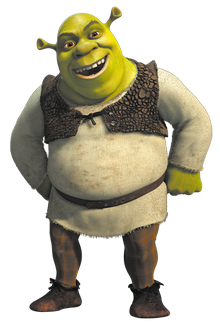
\includegraphics[scale=2]{img/shrek.png}
		\end{figure}

       \vfill
            
   \end{center}
\end{titlepage}

% TODO:
% генерирование n-мерных приколов
% линии уровня


\section{Постановка задания}

Требуется реализовать алгоритмы поиска минимума функции нескольких переменных, исследовать их, оценить поведение:
\begin{itemize}
\item метод градиентного спуска
\item метод наискорейшего спуска
\item метод сопряженных градиентов
\end{itemize}

Ограничение на исследуемые функции -- они должны быть квадратичными, то есть представимы в виде
\[ f(x) = f(x_1, x_2, \cdots, x_n) = \frac{1}{2} \sum_{i, j = 1}^n a_{ij} x_i x_j - \sum_{i=1}^n b_i x_i + c\].

В матричной форме эти функции имеют вид:
\[ f(x) = \frac{1}{2} x^T Ax - b^Tx + c  \text{, где } x = (x_1, \cdots, x_n)^T, b = (b_1, \cdots, b_n)^T \]

\section{Предварительное исследование}

Основная задача -- найти минимум заданной функции. По теореме Ферма, если точка $x^*$ -- минимум функции, то $f'(x^*) = 0$. В многомерном случае можно применить этот критерий последовательно к каждой частной производной, и тогда получится критерий минимума функции нескольких переменных -- равенство всех частных производных нулю. Величина, за это отвечающая -- градиент, то есть если $x^* = (x_1^*, \cdots, x_n^*)$ -- минимум функции, то
\[ \nabla f(x^*) = 0 \]

Рассмотрим частную производную по $x_i$ квадратичной функции:
\[ \frac{\delta}{\delta x_i}f(x_1, \cdots, x_n) = a_{ii}x_i + \sum_{j \neq i} \frac{1}{2} (a_{ij}+a_{ji})x_j - b_i \]

То есть в общем виде градиент квадратичной функции выглядит следующим образом:
\[ \nabla f(x) = Ax-b \]

$A$ -- симметричная матрица ($\Rightarrow$ ее можно рассматривать, как треугольную), у которой на пересечении $i$ строки и $j$ столбца стоит величина $\frac{1}{2}(a_{ij}+a{ji})$.

В случае, если градиент в точке не равен нулю, он показывает направление наибольшего локального увеличения функции. Поэтому, если двигаться в направлении антиградиента (то есть $-\nabla f(x)$), то будет происходить движение в направлении убывания $f(x)$.

\section{Исследуемые функции}

Для анализа методов были выбраны следующие квадратичные функции:

\begin{enumerate}

\item \[ f(x) = 64x_1^2 + 126x_1x_2 + 64x_2^2 - 10x_1 + 30x_2 + 13 \]
\begin{figure}[H]
	\centering
	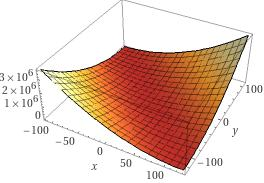
\includegraphics[scale=0.5]{img/func1_plot.jpeg}
	\caption{График функции №1.}
\end{figure}

\begin{figure}[H]
	\centering
	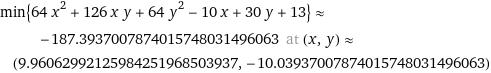
\includegraphics[width=0.5\textwidth]{img/func1_min.jpeg}
	\caption{Минимум, найденный с помощью Wolphram Alpha.}
\end{figure}

\item \[ f(x) = x_1^2+4x_2^2+4x+2y \]
\begin{figure}[H]
	\centering
	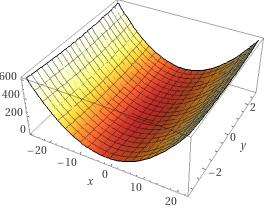
\includegraphics[scale=0.5]{img/func2_plot.jpeg}
	\caption{График функции №2.}
\end{figure}

\begin{figure}[H]
	\centering
	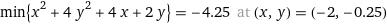
\includegraphics[width=0.5\textwidth]{img/func2_min.jpeg}
	\caption{Минимум, найденный с помощью Wolphram Alpha.}
\end{figure}

\item \[ f(x) = 29x^2+18y^2-8x+10 \]
\begin{figure}[H]
	\centering
	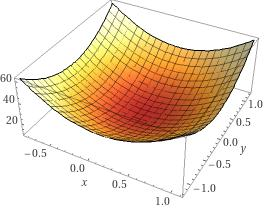
\includegraphics[scale=0.5]{img/func3_plot.jpeg}
	\caption{График функции №3.}
\end{figure}

\begin{figure}[H]
	\centering
	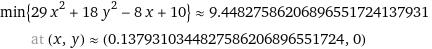
\includegraphics[width=0.5\textwidth]{img/func3_min.jpeg}
	\caption{Минимум, найденный с помощью Wolphram Alpha.}
\end{figure}

\end{enumerate}

\newpage
\section{Метод градиентного спуска}

Как было написано ранее, двигаясь в направлении антиградиента, функция убывает. То есть по точке $x^k$ можно получить точку $x^{k+1}$ с меньшим значением функции $f$. Повторяя это нескольно раз, построится последовательность $x^{k+1} = x^{k} - \alpha^{k} \nabla f(x^k)$. При этом, $\alpha_k$ (величина шага) такова, что $f(x^{k+1}) < f(x^k)$.  

Точка является миниумом, если в ней квадратичная форма положительно определена. Матрица $A$ -- симметричная, будем считать, что положительно определенная. Пусть $L$ -- наибольшее собственное значение $A$, тогда при любых $\alpha \in \left(0; \frac{2}{L} \right)$ и $x$ из области определения фукнции $x^{k+1} = x^{k} - \alpha^{k} \nabla f(x^k)$, будет сходиться к единственной точке глобального минимума $x^*$ линейно, со скоростью геометрической прогрессии. В этом случае последовательность $x_k$ будет релаксационной и не будет происходить "проскакивания" стационарной точки.

Таким образом, посчитав максимальное собственное число $A$, примем $\alpha = \frac{2}{L}$, и затем будем выстраивать последовательность. Если на каком-то шаге $f(x^{k+1}) \geqslant f(x^k)$, то был сделан слишком большой шаг и следует уменьшить $\alpha$. Примем новое $\alpha = \frac{\alpha}{2}$. Будем повторять до условия остановки: $\lVert \nabla f(x^k) \rVert \leqslant \epsilon$, либо до указанного колчиества итераций, если это было дано (в нашем исследовании -- 10000).

\begin{table}[H]
\begin{tabular}{|c|c|c|c|c|c|c|}
\hline
\rowcolor[HTML]{FFF0DB} 
\cellcolor[HTML]{FFF0DB}\textbf{$\epsilon$} &
  \textbf{$x_1$} &
  \textbf{$x_2$} &
  \textbf{\begin{tabular}[c]{@{}c@{}}Кол-во\\ итераций\end{tabular}} &
  \textbf{\begin{tabular}[c]{@{}c@{}}Значение\\ минимума\end{tabular}} &
  \textbf{$x_{1_{min}}$} &
  \textbf{$x_{2_{min}}$} \\ \hline
\rowcolor[HTML]{EDE9E2} 
\multicolumn{7}{|c|}{\cellcolor[HTML]{EDE9E2}$f(x)=64x_1^2+126x_1x_2+64x_2^2-10x_1+30x_2+13$}     \\ \hline
$10^{-2}$ & 10 & 10 & 876   & -187.39370078722567 & 9.9606205571591     & -10.039360714639415     \\ \hline
$10^{-3}$ & 10 & 10 & 876   & -187.39370078722567 & 9.9606205571591     & -10.039360714639415     \\ \hline
$10^{-4}$ & 10 & 10 & 876   & -187.39370078722567 & 9.9606205571591     & -10.039360714639415     \\ \hline
$10^{-5}$ & 10 & 10 & 10000 & -187.3937007873267  & 9.960623763053757   & -10.039363920534072     \\ \hline
$10^{-6}$ & 10 & 10 & 10000 & -187.3937007873267  & 9.960623763053757   & -10.039363920534072     \\ \hline
\rowcolor[HTML]{EDE9E2} 
\multicolumn{7}{|c|}{\cellcolor[HTML]{EDE9E2}$f(x) = x_1^2+4x_2^2+4x+2y$}                         \\ \hline
$10^{-2}$ & 10 & 10 & 29    & -4.249999999999996  & -1.9999999329447746 & -0.25                   \\ \hline
$10^{-3}$ & 10 & 10 & 29    & -4.249999999999996  & -1.9999999329447746 & -0.25                   \\ \hline
$10^{-4}$ & 10 & 10 & 29    & -4.249999999999996  & -1.9999999329447746 & -0.25                   \\ \hline
$10^{-5}$ & 10 & 10 & 29    & -4.249999999999996  & -1.9999999329447746 & -0.25                   \\ \hline
$10^{-6}$ & 10 & 10 & 29    & -4.249999999999996  & -1.9999999329447746 & -0.25                   \\ \hline
\rowcolor[HTML]{FFF0DB} 
\multicolumn{7}{|c|}{\cellcolor[HTML]{EDE9E2}$29x^2+18y^2-8x+10$}                                 \\ \hline
$10^{-2}$ & 10 & 10 & 15    & 9.44827586206899    & 0.137931034482758   & -3.58174971296527E-08   \\ \hline
$10^{-3}$ & 10 & 10 & 15    & 9.44827586206899    & 0.137931034482758   & -3.58174971296527E-08   \\ \hline
$10^{-4}$ & 10 & 10 & 15    & 9.44827586206899    & 0.137931034482758   & -3.58174971296527E-08   \\ \hline
$10^{-5}$ & 10 & 10 & 15    & 9.44827586206899    & 0.137931034482758   & -3.58174971296527E-08   \\ \hline
$10^{-6}$ & 10 & 10 & 16    & 9.448275862068968   & 0.13793103448275862 & -1.3585947187109647E-08 \\ \hline
\end{tabular}
\end{table}

\begin{figure}[H]
	\centering
	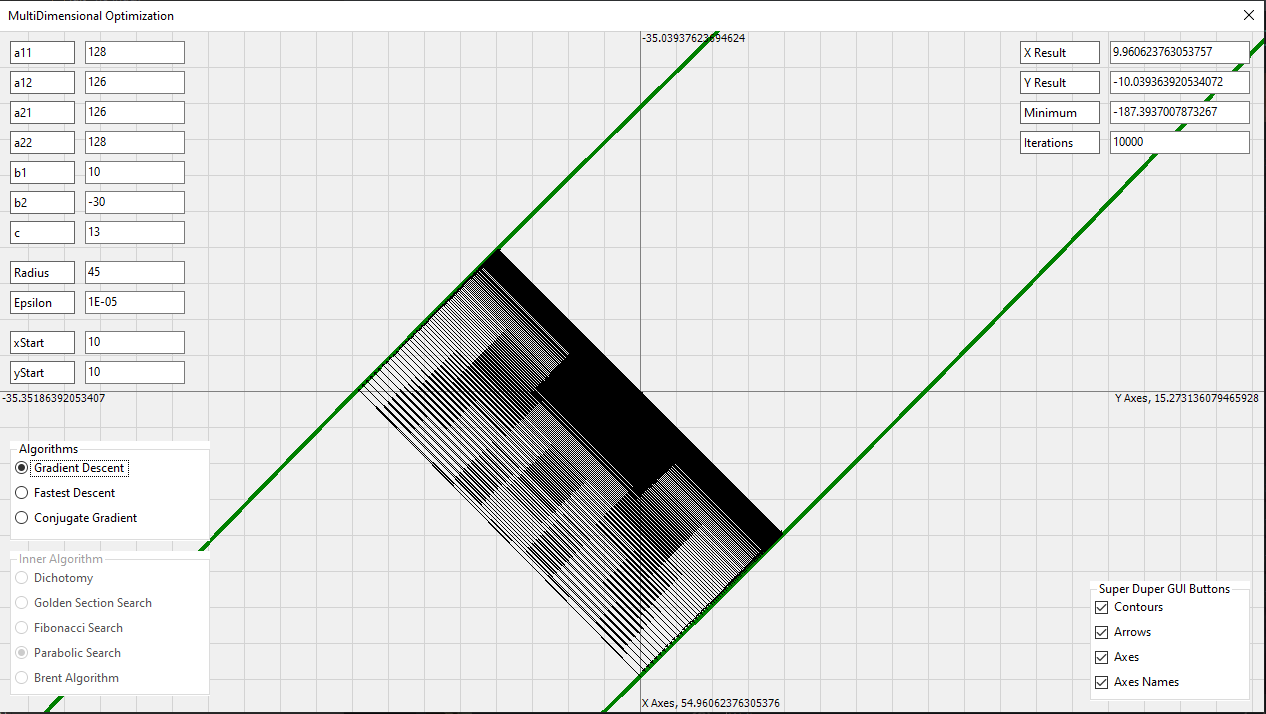
\includegraphics[scale=0.3]{img/1_simp.png}
	\caption{Функция 1}
	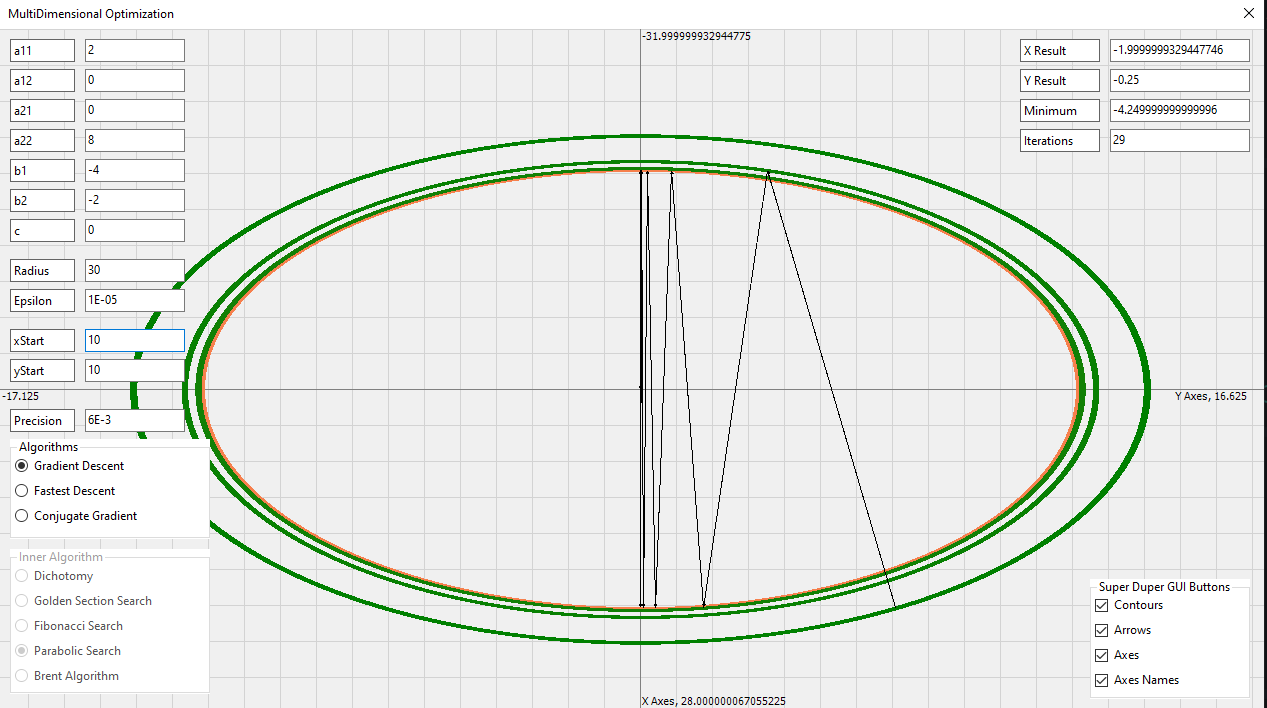
\includegraphics[scale=0.3]{img/2_simp.png}
	\caption{Функция 2}
	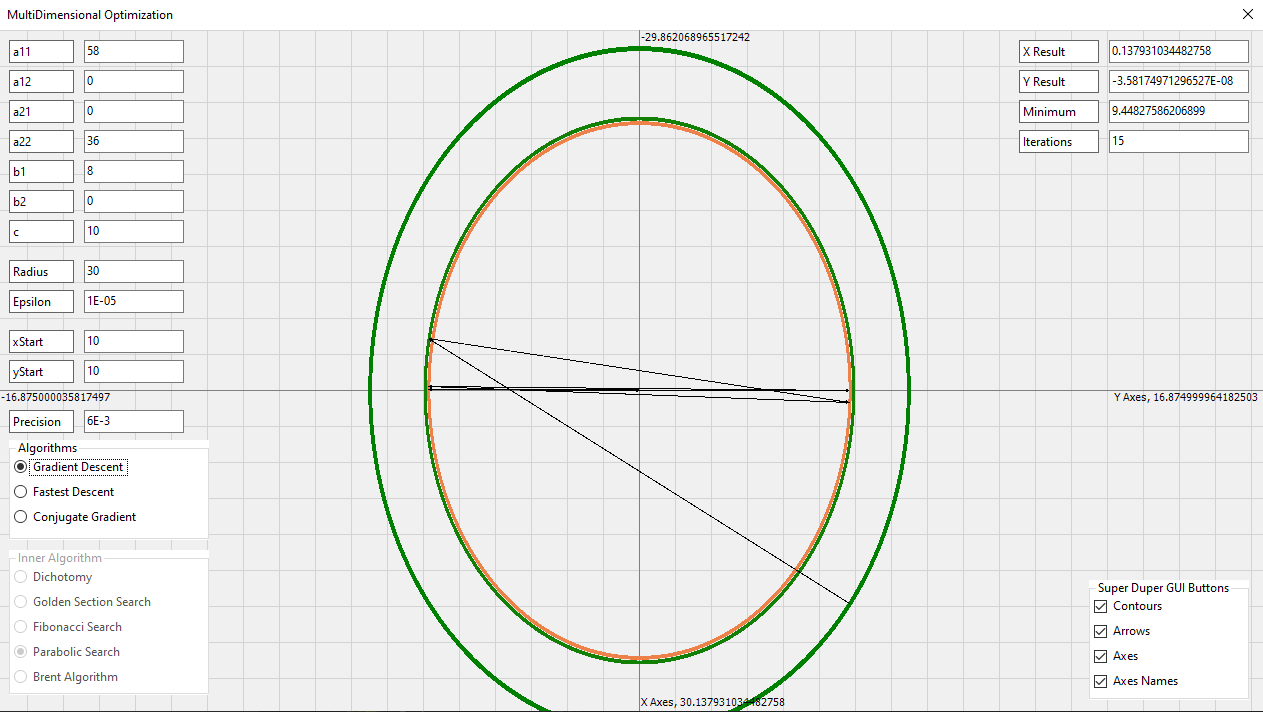
\includegraphics[scale=0.3]{img/3_simp.png}
	\caption{Функция 3}
\end{figure}

\newpage
\section{Метод наискорейшего спуска}

Это модификация предудщего метода, в которой коэффициент $\alpha$ каждый раз пересчитывается. После вычисления в начальной точке градиента, движение в направлении антиградиента делается не маленькими шагами, а до тех пор, пока функция убывает. При достижении минимума на выбранном направлении, снова вычисляется градиент функции и описанные действия повторяются.

На каждом $k$-ом шаге коэффициент $\alpha_k$ находится из решения задачи одномерной оптимизации:
\[ \Phi_k (\alpha_k) \rightarrow min, \quad  \Phi_k (\alpha_k) = f(x^k - \alpha_k \nabla f(x^k)) \]
При этом, $\alpha_k > 0$, поэтому оптимизируем на промежутке $\left[ 0; \frac{2}{L} \right]$.

Таким образом, на каждом шаге будем находить $\alpha_k$, принимать $x^{k+1} = x^{k} - \alpha^{k} \nabla f(x^k)$, до тех пор, пока $\lVert \nabla f(x^k) \rVert \leqslant \epsilon$, либо до указанного колчиества итераций, если это было дано.

\begin{table}[H]
\begin{tabular}{|c|c|c|c|c|c|c|}
\hline
\rowcolor[HTML]{FFF0DB} 
\cellcolor[HTML]{FFF0DB}\textbf{$\epsilon$} &
  \textbf{$x_1$} &
  \textbf{$x_2$} &
  \textbf{\begin{tabular}[c]{@{}c@{}}Кол-во\\ итераций\end{tabular}} &
  \textbf{\begin{tabular}[c]{@{}c@{}}Значение\\ минимума\end{tabular}} &
  \textbf{$x_{1_{min}}$} &
  \textbf{$x_{2_{min}}$} \\ \hline
\rowcolor[HTML]{EDE9E2} 
\multicolumn{7}{|c|}{\cellcolor[HTML]{EDE9E2}$f(x)=64x_1^2+126x_1x_2+64x_2^2-10x_1+30x_2+13$}    \\ \hline
$10^{-2}$ & 10 & 10 & 727  & -187.39367612608606 & 9.957118417601245   & -10.03585857508156      \\ \hline
$10^{-3}$ & 10 & 10 & 698  & -187.39370053896903 & 9.96027747821606    & -10.039017635696377     \\ \hline
$10^{-4}$ & 10 & 10 & 797  & -187.39370078492178 & 9.96059470922056    & -10.039334866700877     \\ \hline
$10^{-5}$ & 10 & 10 & 987  & -187.39370078737676 & 9.960626416187417   & -10.039366573667733     \\ \hline
$10^{-6}$ & 10 & 10 & 1250 & -187.3937007874012  & 9.960629568354005   & -10.039369725834321     \\ \hline
\rowcolor[HTML]{EDE9E2} 
\multicolumn{7}{|c|}{\cellcolor[HTML]{EDE9E2}$f(x) = x_1^2+4x_2^2+4x+2y$}                        \\ \hline
$10^{-2}$ & 10 & 10 & 16   & -4.249988667261994  & -1.9970766063316312 & -0.24916535824055244    \\ \hline
$10^{-3}$ & 10 & 10 & 20   & -4.249999838918146  & -1.9996335176315747 & -0.2499181884365339     \\ \hline
$10^{-4}$ & 10 & 10 & 25   & -4.249999999196022  & -1.999975518591127  & -0.250007152606546      \\ \hline
$10^{-5}$ & 10 & 10 & 29   & -4.24999999998744   & -1.9999969394487098 & -0.25000089350317256    \\ \hline
$10^{-6}$ & 10 & 10 & 34   & -4.249999999999927  & -1.9999997681107133 & -0.24999992938546808    \\ \hline
\rowcolor[HTML]{FFF0DB} 
\multicolumn{7}{|c|}{\cellcolor[HTML]{EDE9E2}$29x^2+18y^2-8x+10$}                                \\ \hline
$10^{-2}$ & 10 & 10 & 7    & 9.448275973454791   & 0.1378722480606154  & -2.4906900895904814E-05 \\ \hline
$10^{-3}$ & 10 & 10 & 9    & 9.448275864130045   & 0.1379268474573064  & 9.287609823917025E-06   \\ \hline
$10^{-4}$ & 10 & 10 & 11   & 9.448275862076303   & 0.1379308093771439  & 5.709298815339414E-07   \\ \hline
$10^{-5}$ & 10 & 10 & 12   & 9.448275862069288   & 0.1379311181748114  & 8.101038924841543E-08   \\ \hline
$10^{-6}$ & 10 & 10 & 14   & 9.448275862068968   & 0.1379310416449409  & 1.0259368808164012E-09  \\ \hline
\end{tabular}
\end{table}

Сравнение количества итераций для внутренних методов одномерной оптимизации (на примере второй функции):

\begin{table}[h]
\centering
\begin{tabular}{|
>{\columncolor[HTML]{EED9C4}}c |c|}
\hline
\cellcolor[HTML]{EDE9E2}\textbf{} & \cellcolor[HTML]{FFF0DB}\textbf{Количество вычислений} \\ \hline
\textbf{Метод дихотомии}        & 600 \\ \hline
\textbf{Метод золотого сечения} & 401 \\ \hline
\textbf{Метод Фибоначчи}        & 426 \\ \hline
\textbf{Метод парабол}          & 125 \\ \hline
\textbf{Метод Брента}           & 311 \\ \hline
\end{tabular}
\end{table}

\begin{figure}[H]
	\centering
	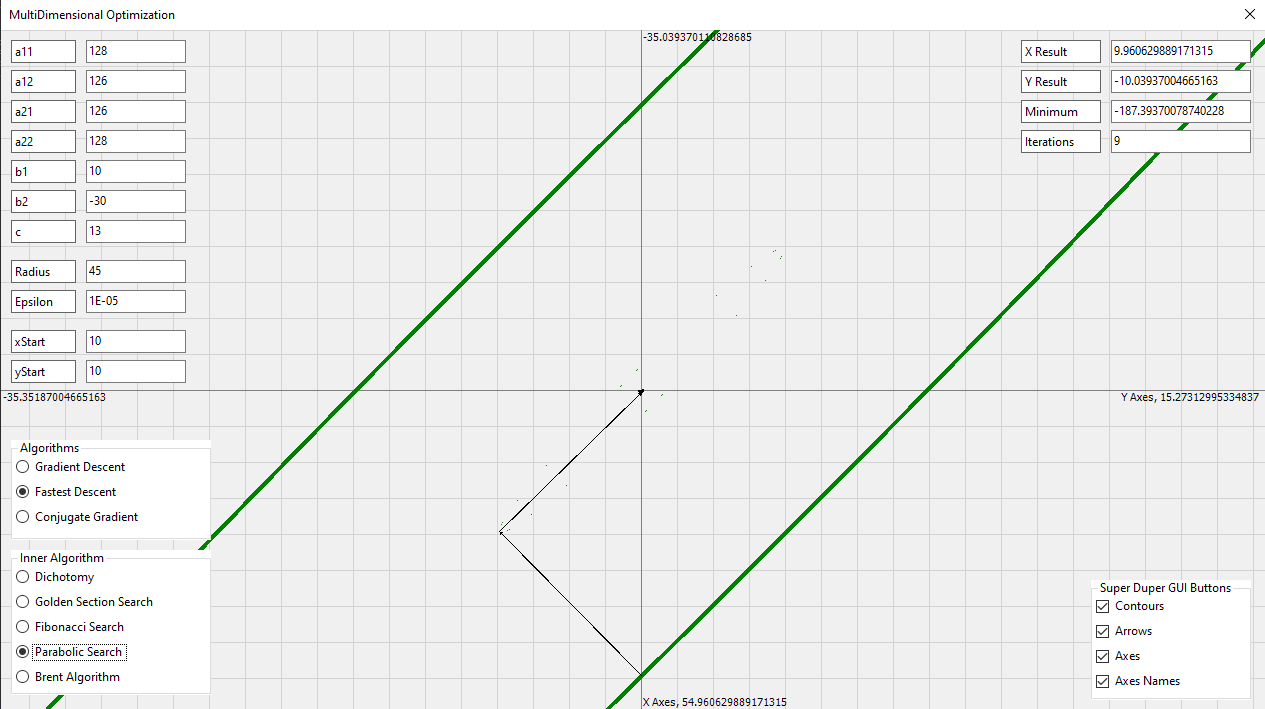
\includegraphics[scale=0.3]{img/1_fd.png}
	\caption{Функция 1}
	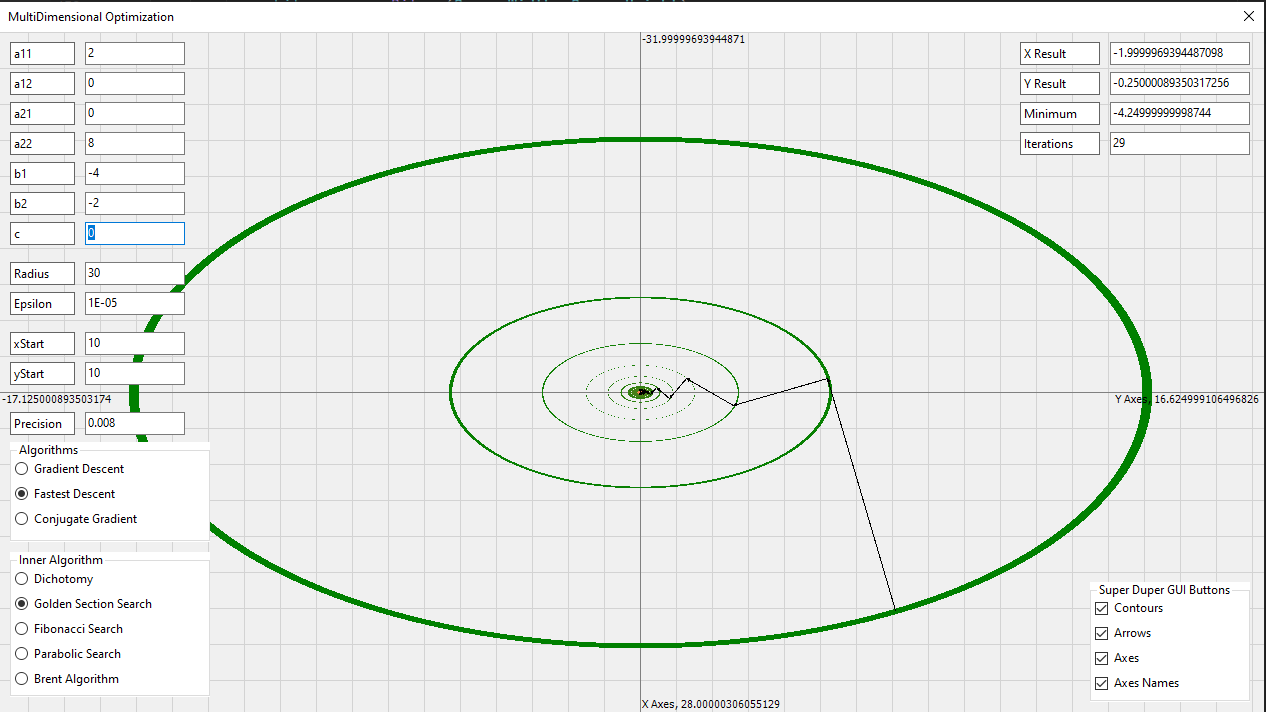
\includegraphics[scale=0.3]{img/2_fd.png}
	\caption{Функция 2}
	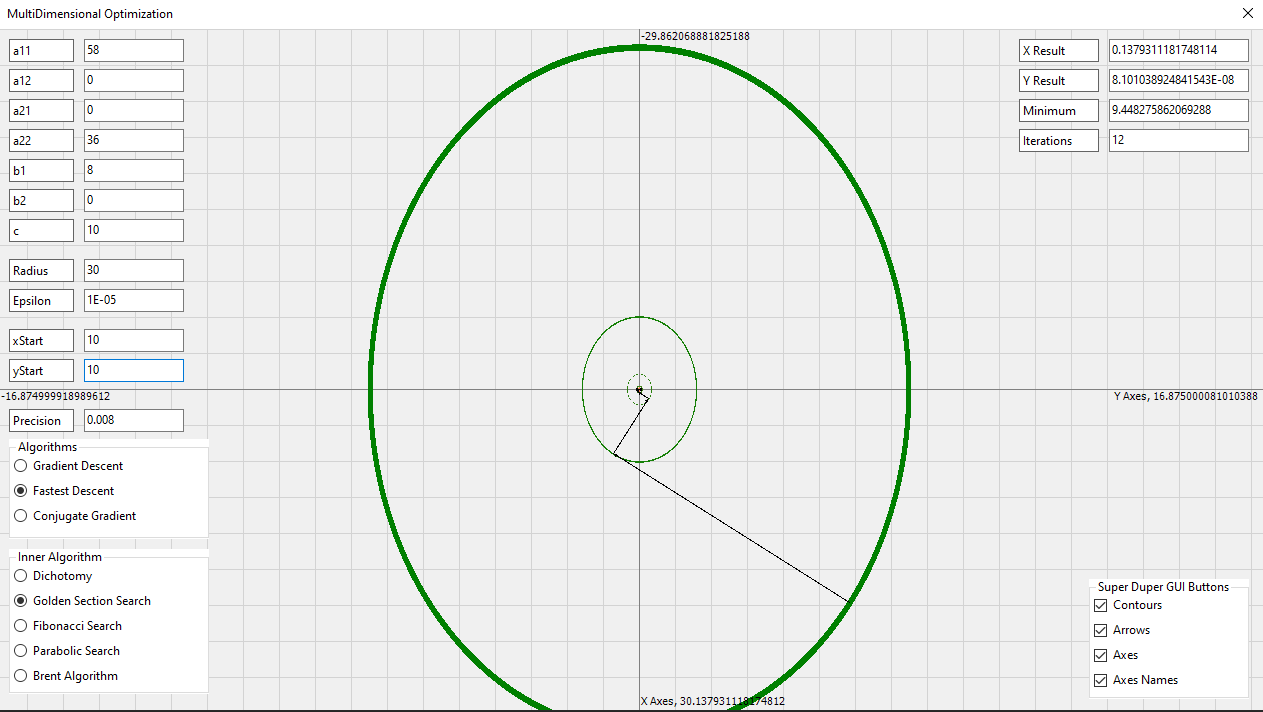
\includegraphics[scale=0.3]{img/3_fd.png}
	\caption{Функция 3}
\end{figure}

\newpage
\section{Метод сопряженных градиентов}

Отличительная особенность данного метода -- он решает квадратичную задачу оптимизации за конечное число шагов (не более, чем $n$ итераций, где $n$ -- размерность пространства).

Рассмотрим ненулевые векторы $p^1, \cdots, p^n$. Они называются сопряженными относительно матрицы $A_{n \times n}$ или А-ортогональными, если для всех $i, j: i \neq j$ выполняется условие $\left(Ap^i, p^j \right) = 0$. Система из таких векторов линейно независима и образует базис в $E_n$. 

Тогда минимизация квадратичной функции $f(x) = \frac{1}{2} \left(Ax, x \right) + \left(b, x \right) + c$ ($A$ -- положительно определенная) сводится к итерационному процессу $x^k=x^{k-1}+\alpha_k p^k$, где $p^k$ -- А-ортогональные. Такой последовательный спуск по А-ортогональным направлениям приводит к точке минимума квадратичной формы не более чем за $n$ шагов. На каждой итерации необходимо выбрать параметры, дающие наилучший многочлен, который можно построить, учитывая все сделанные до текущего шага измерения градиента.

Так как функция квадратичная и есть условие А-ортогональности, нахождение параметров сводится до следующих действий на каждом этапе итераций:

\[ \alpha = \frac{\lVert \nabla f(x^k) \rVert^2}{\left(Ap^k, p^k\right)}, \quad x^{k+1} = x^k+\alpha_k p^k \]
\[ \nabla f(x^{k+1}) = \nabla f(x^k) + \alpha_k Ap^k \]
\[ \beta_k = \frac{\lVert \nabla f(x^{k+1}) \rVert ^2}{\lVert \nabla f(x^{k}) \rVert ^2} \] 
\[ p^{k+1} = -\nabla f(x^{k+1}) + \beta_k p^k \]

\begin{table}[H]
\begin{tabular}{|c|c|c|c|c|c|c|}
\hline
\rowcolor[HTML]{FFF0DB} 
\cellcolor[HTML]{FFF0DB}\textbf{$\epsilon$} &
  \textbf{$x_1$} &
  \textbf{$x_2$} &
  \textbf{\begin{tabular}[c]{@{}c@{}}Кол-во\\ итераций\end{tabular}} &
  \textbf{\begin{tabular}[c]{@{}c@{}}Значение\\ минимума\end{tabular}} &
  \textbf{$x_{1_{min}}$} &
  \textbf{$x_{2_{min}}$} \\ \hline
\rowcolor[HTML]{EDE9E2} 
\multicolumn{7}{|c|}{\cellcolor[HTML]{EDE9E2}$f(x)=64x_1^2+126x_1x_2+64x_2^2-10x_1+30x_2+13$} \\ \hline
$10^{-2}$ & 10 & 10 & 2 & -187.39367612608606 & 9.957118417601245   & -10.03585857508156      \\ \hline
$10^{-3}$ & 10 & 10 & 2 & -187.39370053896903 & 9.96027747821606    & -10.039017635696377     \\ \hline
$10^{-4}$ & 10 & 10 & 2 & -187.39370078492178 & 9.96059470922056    & -10.039334866700877     \\ \hline
$10^{-5}$ & 10 & 10 & 2 & -187.39370078737676 & 9.960626416187417   & -10.039366573667733     \\ \hline
$10^{-6}$ & 10 & 10 & 2 & -187.3937007874012  & 9.960629568354005   & -10.039369725834321     \\ \hline
\rowcolor[HTML]{EDE9E2} 
\multicolumn{7}{|c|}{\cellcolor[HTML]{EDE9E2}$f(x) = x_1^2+4x_2^2+4x+2y$}                     \\ \hline
$10^{-2}$ & 10 & 10 & 2 & -4.249988667261994  & -1.9970766063316312 & -0.24916535824055244    \\ \hline
$10^{-3}$ & 10 & 10 & 2 & -4.249999838918146  & -1.9996335176315747 & -0.2499181884365339     \\ \hline
$10^{-4}$ & 10 & 10 & 2 & -4.249999999196022  & -1.999975518591127  & -0.250007152606546      \\ \hline
$10^{-5}$ & 10 & 10 & 2 & -4.24999999998744   & -1.9999969394487098 & -0.25000089350317256    \\ \hline
$10^{-6}$ & 10 & 10 & 2 & -4.249999999999927  & -1.9999997681107133 & -0.24999992938546808    \\ \hline
\rowcolor[HTML]{FFF0DB} 
\multicolumn{7}{|c|}{\cellcolor[HTML]{EDE9E2}$29x^2+18y^2-8x+10$}                             \\ \hline
$10^{-2}$ & 10 & 10 & 2 & 9.448275973454791   & 0.1378722480606154  & -2.4906900895904814E-05 \\ \hline
$10^{-3}$ & 10 & 10 & 2 & 9.448275864130045   & 0.1379268474573064  & 9.287609823917025E-06   \\ \hline
$10^{-4}$ & 10 & 10 & 2 & 9.448275862076303   & 0.1379308093771439  & 5.709298815339414E-07   \\ \hline
$10^{-5}$ & 10 & 10 & 2 & 9.448275862069288   & 0.1379311181748114  & 8.101038924841543E-08   \\ \hline
$10^{-6}$ & 10 & 10 & 2 & 9.448275862068968   & 0.1379310416449409  & 1.0259368808164012E-09  \\ \hline
\end{tabular}
\end{table}

\begin{figure}[H]
	\centering
	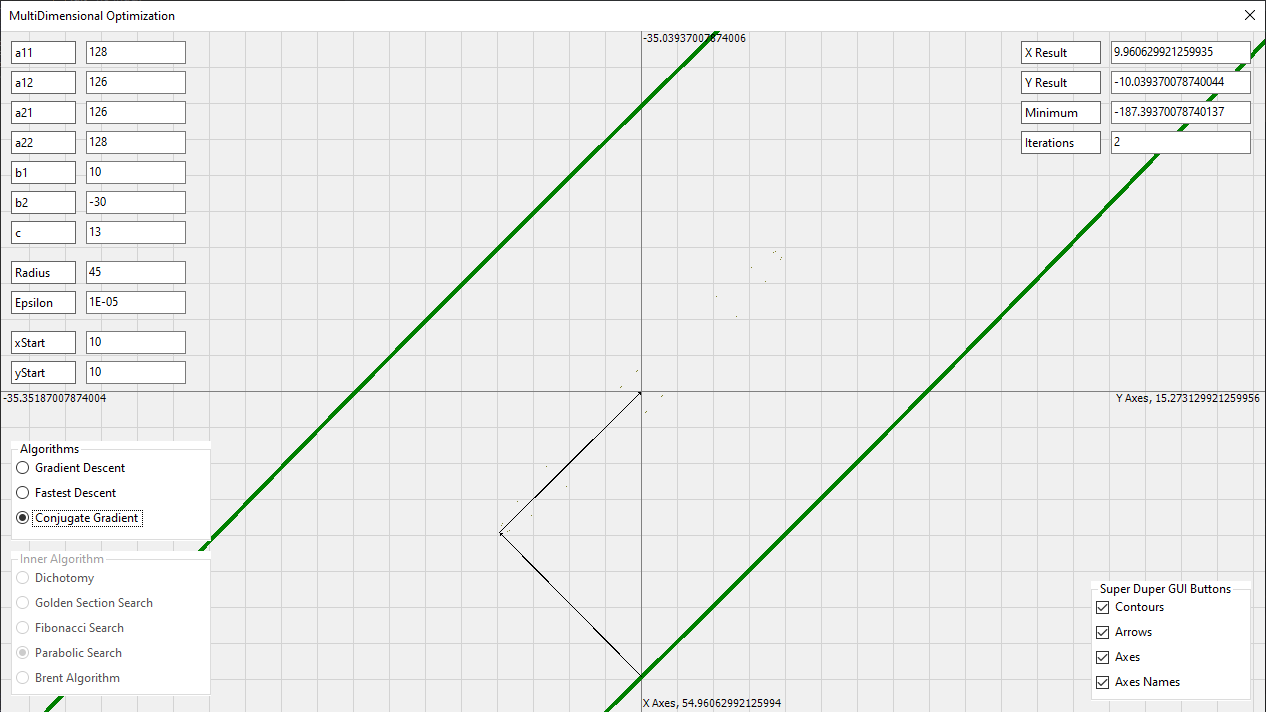
\includegraphics[scale=0.3]{img/1_cd.png}
	\caption{Функция 1}
	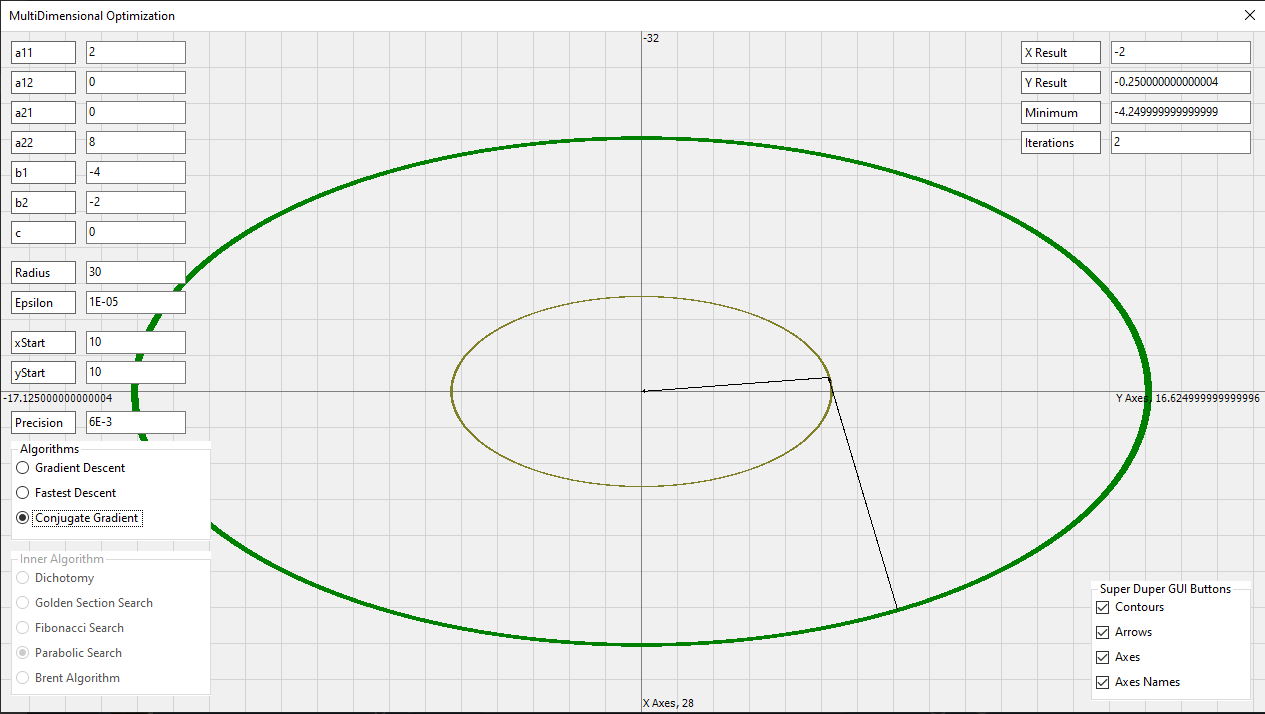
\includegraphics[scale=0.3]{img/2_cd.png}
	\caption{Функция 2}
	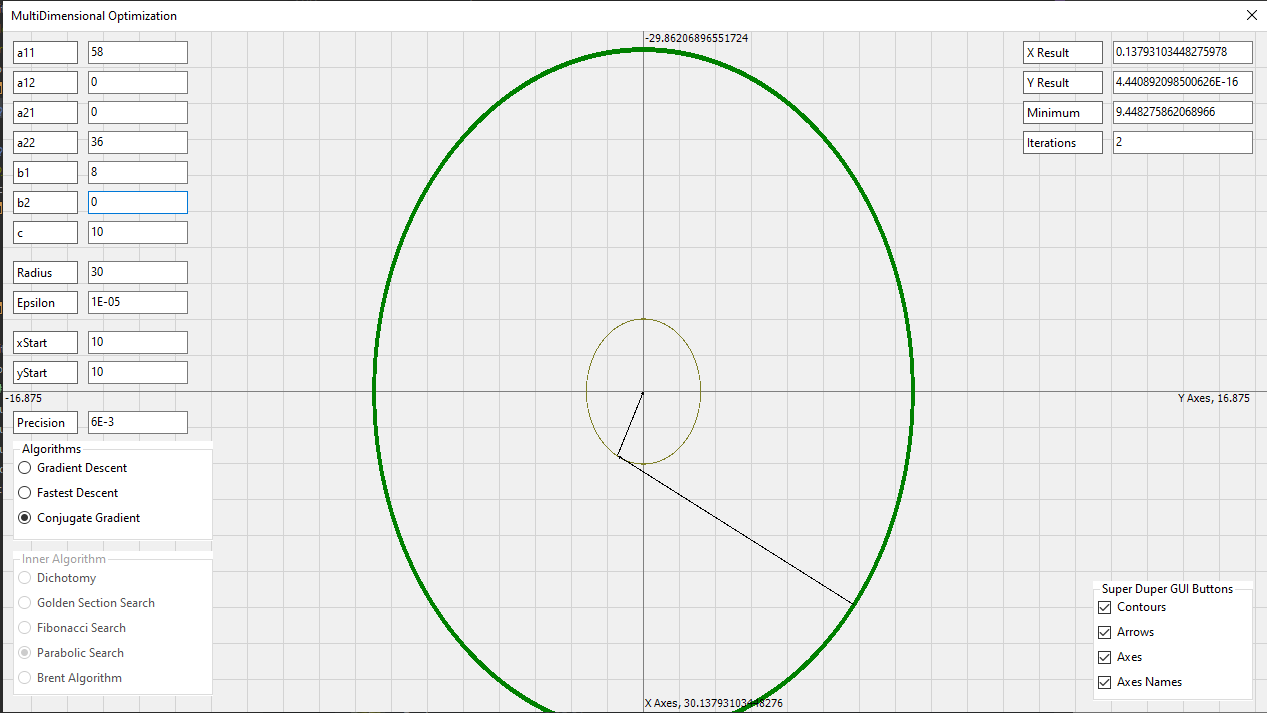
\includegraphics[scale=0.3]{img/3_cd.png}
	\caption{Функция 3}
\end{figure}

\newpage
\section{Сравнение методов}

Для симметричной положительно определенной матрицы число обусловленности $\mu = \frac{L}{l}$, где $L$ -- наибольшее собственное число матрицы $A$, а $l$ -- наименьшее. Оно характеризует степень вытянутости линий уровня $f(x) = const$.

\begin{itemize}
\item Если $\mu$ велико, то линии уровня сильно вытянуты, функция имеет овражный характер, то есть резко меняется по одним направлениям и слабо по другим. В этом случае задача плохо обусловлена.
\item Если $\mu \approx 1$, то линии уровня близки к окружностям и задача является хорошо обсуловленной.
\end{itemize}

Для исследования количества итераций каждого метода на разных числах обсуловленности, будем генерировать квадратичную функцию в виде $a_1 \cdot x_1^2 + \cdots + a_n \cdot x_n^2$, где $a_i > 0$, $a_1$ -- наименьшее число и равно 1, $a_n$ -- наибольшее и равно заданному $k$. У нее положительно определенная матрица с $l = 1, L = k$, а значит $\mu = k$. Также исследуем зависимость от размерности пространства $n$.

Метод градиентного спуска:

\begin{table}[H]
\centering
\begin{tabular}{|
>{\columncolor[HTML]{EED9C4}}c |c|c|c|c|c|c|c|c|c|c|}
\hline
\cellcolor[HTML]{EDE9E2}\textbf{$n$ / $k$} &
  \cellcolor[HTML]{FFF0DB}\textbf{10} &
  \cellcolor[HTML]{FFF0DB}\textbf{50} &
  \cellcolor[HTML]{FFF0DB}\textbf{100} &
  \cellcolor[HTML]{FFF0DB}\textbf{200} &
  \cellcolor[HTML]{FFF0DB}\textbf{400} &
  \cellcolor[HTML]{FFF0DB}\textbf{600} &
  \cellcolor[HTML]{FFF0DB}\textbf{800} &
  \cellcolor[HTML]{FFF0DB}\textbf{1000} &
  \cellcolor[HTML]{FFF0DB}\textbf{1250} &
  \cellcolor[HTML]{FFF0DB}\textbf{1500} \\ \hline
\textbf{2}     & 79 & 372 & 708 & 1355 & 2567 & 3796 & 4863 & 6016 & 7446  & 8647  \\ \hline
\textbf{10}    & 84 & 372 & 708 & 1355 & 2567 & 3796 & 4863 & 6016 & 7446  & 8647  \\ \hline
\textbf{50}    & 88 & 379 & 740 & 1355 & 2567 & 3796 & 4863 & 6016 & 7446  & 8647  \\ \hline
\textbf{100}   & 89 & 419 & 746 & 1355 & 2567 & 3796 & 4863 & 6016 & 7446  & 8647  \\ \hline
\textbf{250}   & 91 & 438 & 825 & 1434 & 2567 & 3796 & 5073 & 6187 & 7446  & 10000 \\ \hline
\textbf{500}   & 92 & 447 & 863 & 1651 & 3167 & 3796 & 6341 & 6016 & 9677  & 10000 \\ \hline
\textbf{750}   & 94 & 454 & 870 & 1722 & 3232 & 4758 & 6194 & 7909 & 9682  & 8647  \\ \hline
\textbf{1000}  & 93 & 455 & 870 & 1652 & 3232 & 4859 & 6473 & 6016 & 7675  & 8647  \\ \hline
\textbf{1500}  & 95 & 463 & 892 & 1709 & 3234 & 4860 & 6199 & 8023 & 10000 & 8902  \\ \hline
\textbf{10000} & 99 & 487 & 935 & 1820 & 3484 & 5219 & 6613 & 8239 & 10000 & 10000 \\ \hline
\end{tabular}
\end{table}

\begin{figure}[H]
	\centering
	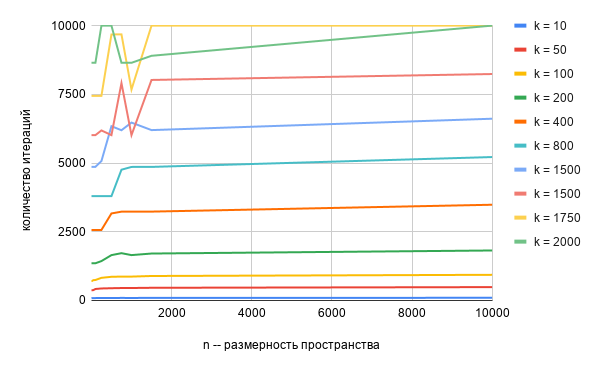
\includegraphics[scale=0.5]{img/chart_simp.png}
\end{figure}

Метод наискорейшего спуска:

\begin{table}[H]
\centering
\begin{tabular}{|
>{\columncolor[HTML]{EED9C4}}c |c|c|c|c|c|c|c|c|c|c|}
\hline
\cellcolor[HTML]{EDE9E2}\textbf{$n$ / $k$} &
  \cellcolor[HTML]{FFF0DB}\textbf{10} &
  \cellcolor[HTML]{FFF0DB}\textbf{50} &
  \cellcolor[HTML]{FFF0DB}\textbf{100} &
  \cellcolor[HTML]{FFF0DB}\textbf{200} &
  \cellcolor[HTML]{FFF0DB}\textbf{400} &
  \cellcolor[HTML]{FFF0DB}\textbf{600} &
  \cellcolor[HTML]{FFF0DB}\textbf{800} &
  \cellcolor[HTML]{FFF0DB}\textbf{1000} &
  \cellcolor[HTML]{FFF0DB}\textbf{1250} &
  \cellcolor[HTML]{FFF0DB}\textbf{1500} \\ \hline
\textbf{2}     & 59 & 283 & 593 & 1154 & 2323 & 3510 & 4732 & 5917 & 7531 & 9038  \\ \hline
\textbf{10}    & 61 & 307 & 595 & 1156 & 2324 & 3511 & 4733 & 5918 & 7531 & 9039  \\ \hline
\textbf{50}    & 64 & 299 & 595 & 1156 & 2324 & 3511 & 4733 & 5918 & 7531 & 9038  \\ \hline
\textbf{100}   & 67 & 307 & 613 & 1156 & 2324 & 3511 & 4733 & 5917 & 7531 & 9310  \\ \hline
\textbf{250}   & 68 & 322 & 630 & 1190 & 2324 & 3510 & 4733 & 5917 & 7531 & 9038  \\ \hline
\textbf{500}   & 69 & 322 & 652 & 1210 & 2434 & 3510 & 4733 & 5917 & 7531 & 9038  \\ \hline
\textbf{750}   & 70 & 338 & 650 & 1245 & 2394 & 3616 & 4959 & 5917 & 7890 & 9038  \\ \hline
\textbf{1000}  & 71 & 336 & 661 & 1245 & 2486 & 3722 & 4875 & 5917 & 7531 & 9469  \\ \hline
\textbf{1500}  & 72 & 339 & 664 & 1284 & 2486 & 3722 & 5018 & 5917 & 7531 & 9310  \\ \hline
\textbf{10000} & 76 & 364 & 711 & 1352 & 2652 & 3923 & 5064 & 6576 & 8284 & 10000 \\ \hline
\end{tabular}
\end{table}

\begin{figure}[H]
	\centering
	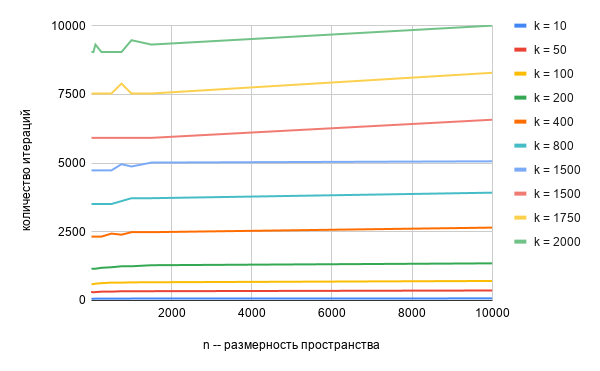
\includegraphics[scale=0.5]{img/chart_fast.png}
\end{figure}

Метод сопряженных градиентов:

\begin{table}[H]
\centering
\begin{tabular}{|
>{\columncolor[HTML]{EED9C4}}c |c|c|c|c|c|c|c|c|c|c|}
\hline
\cellcolor[HTML]{EDE9E2}\textbf{$n$ / $k$} &
  \cellcolor[HTML]{FFF0DB}\textbf{10} &
  \cellcolor[HTML]{FFF0DB}\textbf{50} &
  \cellcolor[HTML]{FFF0DB}\textbf{100} &
  \cellcolor[HTML]{FFF0DB}\textbf{200} &
  \cellcolor[HTML]{FFF0DB}\textbf{400} &
  \cellcolor[HTML]{FFF0DB}\textbf{600} &
  \cellcolor[HTML]{FFF0DB}\textbf{800} &
  \cellcolor[HTML]{FFF0DB}\textbf{1000} &
  \cellcolor[HTML]{FFF0DB}\textbf{1250} &
  \cellcolor[HTML]{FFF0DB}\textbf{1500} \\ \hline
\textbf{2}     & 2  & 2  & 2  & 2  & 2   & 2   & 2   & 2   & 2   & 2   \\ \hline
\textbf{10}    & 6  & 10 & 9  & 10 & 10  & 10  & 10  & 10  & 10  & 10  \\ \hline
\textbf{50}    & 10 & 27 & 27 & 38 & 34  & 46  & 43  & 35  & 45  & 40  \\ \hline
\textbf{100}   & 10 & 35 & 36 & 41 & 60  & 74  & 58  & 62  & 56  & 58  \\ \hline
\textbf{250}   & 10 & 36 & 53 & 74 & 71  & 84  & 99  & 91  & 102 & 88  \\ \hline
\textbf{500}   & 10 & 37 & 54 & 67 & 100 & 85  & 101 & 112 & 101 & 137 \\ \hline
\textbf{750}   & 10 & 37 & 54 & 77 & 97  & 109 & 146 & 141 & 172 & 145 \\ \hline
\textbf{1000}  & 10 & 37 & 54 & 78 & 110 & 133 & 141 & 133 & 160 & 144 \\ \hline
\textbf{1500}  & 10 & 38 & 55 & 78 & 110 & 126 & 157 & 168 & 168 & 178 \\ \hline
\textbf{10000} & 10 & 38 & 56 & 81 & 115 & 140 & 162 & 181 & 202 & 221 \\ \hline
\end{tabular}
\end{table}

\begin{figure}[H]
	\centering
	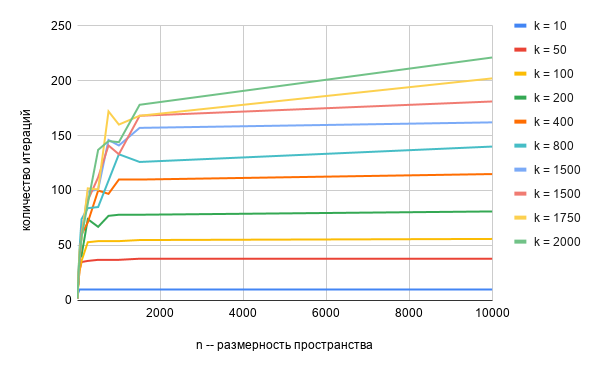
\includegraphics[scale=0.5]{img/chart_conj.png}
\end{figure}

\section{Выводы}

Метод сопряженных градиентов показал себя наилучшим образом -- ему требуется малое количество итераций, однако при его реализации требуются различные вычислительные оптимизации, которые сильно зависят от вида функции нескольких переменных. Также производится несколько вычислений. На различных $n$ и $\mu$ ведет себя относительно стабильно, почти без резких скачков.

Метод градиентного спуска прост в реализации, не требует затратных вычислений и применения одномерных оптимизаций. Однако, ему требуется наибольшее количество итераций, так как происходит движение по ломаной (зигзагом), а не ищется более оптимальная. Также, на различных $n$ и $\mu$ ведет себя нестабильнее всех, совершая резкие скачки на больших $\mu$.

Метод наискорейшего спуска требует меньшего количества итераций, однако внутри происходит вычисление минимума при помощи методов одномерной оптимизации, которые затрачивают итерации. Исходя из замеров, внутренний метод парабол ведет себя лучше остальных методов одномерной оптимизации, требуя меньшего количества как итераций, так и вычислений в целом. 

Реализация: \href{https://github.com/Mr3zee/ITMO-Optimization-Methods-LAB2-2021/}{GitHub}.

\end{document}